\documentclass[journal]{IEEEtran}

\usepackage{amsmath,amsfonts,amssymb}
\usepackage{algorithm}
\usepackage{algorithmic}
\usepackage{array}
\usepackage[caption=false,font=normalsize,labelfont=sf,textfont=sf]{subfig}
\usepackage{textcomp}
\usepackage{stfloats}
\usepackage{url}
\usepackage{verbatim}
\usepackage{graphicx}
\usepackage{cite}
\usepackage{booktabs}
\usepackage{xeCJK}
\usepackage{float}
\usepackage{placeins}

\setmainfont{Times New Roman}
\setsansfont{Arial}
\setmonofont{Courier New}
\setCJKmainfont{SimSun}[BoldFont=SimHei,ItalicFont=KaiTi,SmallCapsFont=SimSun]
\setCJKsansfont{SimHei}
\setCJKmonofont{SimSun}
\raggedbottom

\begin{document}

\title{面向视觉伺服反无人机系统时延补偿的轻量因果时序网络控制参考信号预测方法}

\author{赵龙坤%
\thanks{稿件收到日期：2026年X月X日；修订日期：2026年X月X日。}}

\markboth{IEEE Transactions on Control Systems Technology,~Vol.~XX, No.~X, XXXX~2026}%
{赵龙坤: 面向视觉伺服反无人机系统时延补偿的因果时序控制参考信号预测方法}

\maketitle

\begin{abstract}
视觉伺服反无人机系统通常需要根据目标检测结果实时生成云台或电机控制参考量。然而，从相机采集、图像传输到目标检测推理及后续滤波整形之间存在不可忽略的处理时延，使控制链获得的信息相对于目标真实运动存在一帧级滞后。针对该问题，本文不直接从原始图像端到端生成执行器命令，而是在保留已有稳定基线控制链的基础上，将时延补偿表述为严格因果条件下的基线控制参考信号一帧超前预测问题。具体而言，本文以工程日志中的 \texttt{first\_filter\_dx}/\texttt{first\_filter\_dy} 作为 legacy control reference；该信号由检测框中心坐标经卡尔曼滤波、相机中心偏差计算、阶跃限幅和低通滤波后得到，具有较好的平滑性和工程可用性，但仍包含视觉处理链路带来的短时滞后。为预测下一帧基线控制参考，本文提出 DSCGNet，一种轻量质量感知双流因果时序网络。该网络分别对 $x/y$ 两轴的历史控制参考、一阶差分和二阶差分进行因果建模，并通过质量分支引入检测置信度、目标尺度、丢帧标记和时间间隔等信息；输出端采用有界状态转移参数化形式，使预测值以当前稳定控制参考为基准生成受限增量。实验数据采集自真实二维转台视觉伺服反无人机系统运行日志。信号级评估结果表明，所提方法在 Ahead MAE 和 Ahead RMSE 上优于 Last Value、Linear Extrapolation、Kalman CV 和 GRU Direct 等基线，同时保持较低的补偿增量抖动和方向未跟随率，说明其具有作为实时视觉伺服时延补偿模块的潜力。
\end{abstract}

\begin{IEEEkeywords}
视觉伺服，反无人机系统，时延补偿，因果时序预测，控制参考信号，轻量网络
\end{IEEEkeywords}

\section{引言}
视觉伺服反无人机系统是低空目标监视、跟踪与拦截任务中的重要组成部分\cite{chaumette2006visual,hutchinson1996tutorial,corke2011robotics,shi2021anti}。在此类系统中，目标检测算法输出的无人机检测框中心坐标通常被转换为图像平面上的二维偏差，并进一步映射为云台或电机控制参考量。因此，感知信息的及时性、稳定性和可用性会直接影响执行机构的跟踪响应。

实际工程系统通常不会直接将原始检测框中心偏差送入执行端，而是先对检测框中心坐标进行状态估计与信号整形。例如，检测结果可先经卡尔曼滤波获得较平滑的位置与速度估计，再与摄像头图像中心相减，并经过阶跃限幅与低通滤波形成较稳定的二维控制参考信号\cite{yilmaz2006object,kalman1960new,welch1995introduction}。这一基线控制链能够抑制检测框尺度突变、局部误检和中心坐标抖动带来的高频波动，为执行器提供相对平滑的输入。然而，该链路本身仍需要经历相机采图、数据传输、目标检测推理和滤波整形等环节；当目标快速机动时，控制参考量会不可避免地落后于目标真实状态。

从感知侧看，Faster R-CNN、YOLO、DETR 以及 ResNet 等检测和特征提取方法为视觉目标检测与跟踪提供了重要基础\cite{redmon2016you,he2016deep,ren2015faster,bochkovskiy2020yolov4,carion2020detr}，相关中文综述也系统总结了视觉目标检测和无人机视角目标检测的技术进展\cite{cao2022survey_cn,leng2023droneview_cn}。但是，本文关注的重点并不是改进检测器本身，而是在已有检测与控制链稳定工作的前提下，缓解视觉处理链路带来的短时控制滞后。对反无人机场景而言，即便一帧级时延的绝对时间只有数十毫秒，也可能导致云台始终追随上一拍的目标位置，进而引起动态响应变慢和跟踪误差增大。

传统时延补偿方法通常依赖显式系统模型或状态空间假设。Smith 预测器\cite{smith1957closer}和模型预测控制\cite{camacho2013model}可在具有较准确模型的条件下处理时延问题，但视觉伺服反无人机系统同时受到目标机动、检测质量变化、漏检和执行机构动态的影响，难以建立精确统一的解析模型。另一方面，滑动平均、低通滤波和卡尔曼滤波等方法可以提高信号平滑性，但它们的主要目标是去噪和估计，而不是直接给出下一帧可用的控制参考。

近年来，深度学习时序模型在序列预测任务中表现突出\cite{lecun2015deep}。循环神经网络如 LSTM\cite{hochreiter1997long}和 GRU\cite{cho2014learning}能够捕获时序依赖，时序卷积网络（TCN）\cite{bai2018empirical}通过因果卷积实现高效建模，注意力机制也被广泛用于长序列建模\cite{vaswani2017attention,lim2021tft,wen2023transformers}。然而，如果将控制参考预测简单视为普通时间序列未来值回归，模型容易只追求数值误差最小，而忽略控制链路所要求的严格因果性、输出平滑性、增量受限和实时部署约束。

基于上述考虑，本文提出一种面向视觉伺服反无人机系统短时滞后补偿的轻量因果时序预测方法。本文方法不替代原有稳定控制链，也不从原始图像直接生成电机命令，而是学习已有基线控制参考信号的下一帧输出。本文的主要贡献如下：
\begin{itemize}
    \item 将视觉伺服反无人机系统中的一帧时延补偿问题表述为 legacy control reference 的严格因果 one-step-ahead prediction，使学习目标直接对应已有工程控制链中的稳定参考量。
    \item 提出 DSCGNet，一种轻量质量感知双流因果时序网络，分别对 $x/y$ 两轴控制参考及其一、二阶差分进行建模，并利用检测质量特征刻画当前观测可靠性。
    \item 设计有界状态转移参数化输出头，使模型以当前基线控制参考为锚点预测受限增量，而非无约束直接回归下一帧绝对控制量，从而增强输出的控制友好性。
    \item 基于真实二维转台视觉伺服反无人机系统日志进行信号级验证，并与 Last Value、Linear Extrapolation、Kalman CV 和 GRU Direct 等基线进行比较，同时分析历史长度、质量分支、因果注意力和输出参数化的影响。
\end{itemize}

\section{相关工作}

\subsection{视觉伺服控制信号与状态估计}
视觉伺服控制的核心在于利用视觉反馈实时修正执行机构状态\cite{chaumette2006visual,hutchinson1996tutorial}。在实际系统中，检测框中心坐标通常存在抖动、误检、漏检和尺度突变，因此需要状态估计与信号滤波提高控制输入的可用性。卡尔曼滤波\cite{kalman1960new,welch1995introduction}是一类经典状态估计方法，常用于从噪声观测中递推估计目标位置和速度。经典 PID 及其改进策略仍然是许多工程控制链路中的基本组成部分\cite{liu2003advancedpid}。本文继承这一工程思路：首先保留已有滤波、限幅和低通整形得到的稳定基线控制参考，然后在其上叠加数据驱动的一帧前瞻预测模块。

\subsection{时延补偿方法}
控制系统中的时延补偿是经典问题。Smith 预测器\cite{smith1957closer}通过构建被控对象模型预测未来状态，模型预测控制\cite{camacho2013model}则通过滚动优化未来时域内的控制序列处理时延和约束。围绕显式时滞补偿、约束 MPC 以及带饱和环节的控制对象，已有研究给出了系统分析\cite{normey2009taking,xi2013mpc_cn,li2006saturatedmpc_cn,chen2007timedelaympc_cn}。这些方法在模型较准确时具有清晰理论基础，但在视觉伺服反无人机场景中，感知链路、目标运动和执行机构动态均存在不确定性，直接建立精确模型较困难。本文采用模型无关的信号级预测思路，以已有基线控制参考为监督目标，降低接入风险。

\subsection{深度学习时序预测}
LSTM\cite{hochreiter1997long}、GRU\cite{cho2014learning}、TCN\cite{bai2018empirical}和 WaveNet\cite{oord2016wavenet}等模型已广泛用于序列建模。DA-RNN\cite{qin2017darnn}、Temporal Fusion Transformer\cite{lim2021tft}和 Transformer\cite{vaswani2017attention}进一步利用注意力机制增强长时依赖建模能力，相关综述总结了深度时序预测模型的适用性与局限\cite{wen2023transformers}。与通用时间序列预测不同，本文任务需要满足在线控制中的严格因果性和输出约束。因此，本文采用轻量因果卷积、GRU 和因果注意力组合，并在输出端引入有界状态转移，使网络预测值更适合与已有控制链融合。

\section{问题描述与因果时间对齐}

\subsection{基线控制参考信号定义}
设时刻 $t$ 目标检测算法输出的检测框中心坐标为 $c(t)=[x_c(t),y_c(t)]^T$。实际系统首先对目标中心坐标进行二维卡尔曼滤波，得到平滑中心坐标和速度估计：
\begin{equation}
\hat{c}(t)=[\hat{x}_c(t),\hat{y}_c(t)]^T,\quad
\hat{v}(t)=[\hat{v}_x(t),\hat{v}_y(t)]^T .
\end{equation}
设相机图像中心为 $c_{cam}=[x_{cam},y_{cam}]^T$，则滤波后的图像平面偏差为
\begin{equation}
e_f(t)=\hat{c}(t)-c_{cam}=[e_x(t),e_y(t)]^T .
\end{equation}
其中 $e_x(t)$ 和 $e_y(t)$ 分别表示目标相对于图像中心在水平和垂直方向上的偏差。

为抑制偶发大跳变，对 $e_f(t)$ 施加逐轴阶跃限幅：
\begin{equation}
\tilde{e}(t)=\tilde{e}(t-1)+\mathrm{clip}\!\left(e_f(t)-\tilde{e}(t-1),-k_{\max},k_{\max}\right),
\end{equation}
其中 $k_{\max}$ 为单帧最大允许变化幅度，$\mathrm{clip}(\cdot)$ 按轴逐元素作用。随后对 $\tilde{e}(t)$ 进行低通滤波，得到基线控制参考信号
\begin{equation}
u^L(t)=[u_x^L(t),u_y^L(t)]^T=\mathrm{LPF}(\tilde{e}(t)).
\end{equation}
工程日志字段 \texttt{first\_filter\_dx} 和 \texttt{first\_filter\_dy} 分别对应 $u_x^L(t)$ 和 $u_y^L(t)$。下文将 $u^L(t)$ 称为基线控制参考信号，也称为 legacy control reference/signal。该信号是已有工程链路中经过滤波和限制后的稳定参考量，而不是原始检测框中心坐标。

\subsection{一帧滞后与信号可用性}
视觉伺服链路中的一帧级滞后主要来自相机采集、图像传输、目标检测推理以及控制信号整形等环节。相机工作在约 30\,FPS 时，单帧周期约为 33\,ms；结合系统链路分析，从图像采集到生成可用控制参考的综合时延约为 50\,ms。若能在严格因果条件下根据当前及历史可用信号预测下一帧基线控制参考，则可对其中约一个帧周期的滞后进行前瞻补偿，使有效剩余滞后降至约 $50-33=17$\,ms。该数值是基于当前系统帧率和链路时延的工程估计，用于说明一帧预测在本系统中的时间尺度意义。

为了避免未来信息泄漏，本文显式区分信号索引与在线可用性。定义 $\mathcal{A}_t$ 为模型在控制更新时刻 $t$ 已经可获得的信息集合，则
\begin{equation}
\mathcal{A}_t=\left\{u^L(i),q(i)\mid i\leq t\right\},
\end{equation}
其中 $q(i)$ 为第 $i$ 个时刻的检测质量相关特征。DSCGNet 在时刻 $t$ 的输入仅由 $\mathcal{A}_t$ 中长度为 $T$ 的历史窗口构成：
\begin{equation}
\mathbf{X}_{t}=[\mathbf{x}_{t-T+1},\ldots,\mathbf{x}_{t}],
\end{equation}
并输出对下一帧基线控制参考的预测 $\hat{u}^L(t+1)$。训练时使用 $u^L(t+1)$ 作为监督目标，但推理时模型不访问 $u^L(t+1)$ 或任何未来检测结果。

表\ref{tab:causal_timing}给出了本文采用的因果时间对齐关系。该表强调：模型输入窗口中的所有信号均在时刻 $t$ 已经由旧控制链产生，预测目标 $u^L(t+1)$ 仅在离线训练和评估中作为标签使用。

\begin{table}[!t]
\centering
\caption{因果时间对齐与信号可用性}
\label{tab:causal_timing}
\small
\setlength{\tabcolsep}{3pt}
\resizebox{\columnwidth}{!}{%
\begin{tabular}{lll}
\toprule
\textbf{项目} & \textbf{时刻 $t$ 可用性} & \textbf{用途} \\
\midrule
$u^L(t-T+1),\ldots,u^L(t)$ & 已可用 & 模型历史输入 \\
$q(t-T+1),\ldots,q(t)$ & 已可用 & 质量分支输入 \\
$\hat{u}^L(t+1)$ & 由模型在时刻 $t$ 生成 & 一帧前瞻控制参考 \\
$u^L(t+1)$ & 时刻 $t$ 不可用 & 离线训练/评估标签 \\
\bottomrule
\end{tabular}%
}
\end{table}

\subsection{任务定义}
本文任务是在时刻 $t$ 仅利用当前及过去已经可获得的信息，预测下一帧基线控制参考：
\begin{equation}
\hat{u}^L(t+1)=f_\theta(\mathbf{X}_t),\quad \mathbf{X}_t\subset\mathcal{A}_t.
\end{equation}
理想输出应满足以下要求：
\begin{itemize}
    \item \textbf{前瞻性}：尽量逼近下一帧基线控制参考 $u^L(t+1)$，为一帧时延补偿提供可用信号；
    \item \textbf{因果性}：输入窗口不包含未来帧检测结果或未来控制参考；
    \item \textbf{控制友好性}：输出相对当前参考 $u^L(t)$ 的变化应受限且平滑，避免执行端产生不必要突变；
    \item \textbf{可部署性}：模型计算开销应远小于视觉处理链路的一帧时间尺度。
\end{itemize}

\section{所提方法}

\subsection{总体框架}
本文提出的 DSCGNet 是一个可端到端训练的轻量因果时序预测模块。它并不替代目标检测器、卡尔曼滤波器或底层执行器控制器，而是接在已有基线控制链之后，根据最近 $T$ 帧基线控制参考及质量特征预测下一帧基线控制参考。整体流程如图\ref{fig:method_overview}所示，可分为两级：第一级由旧控制链生成稳定但滞后的 $u^L(t)$；第二级由 DSCGNet 进行严格因果的一帧超前预测，输出 $\hat{u}^L(t+1)$。

\begin{figure*}[!t]
\centering
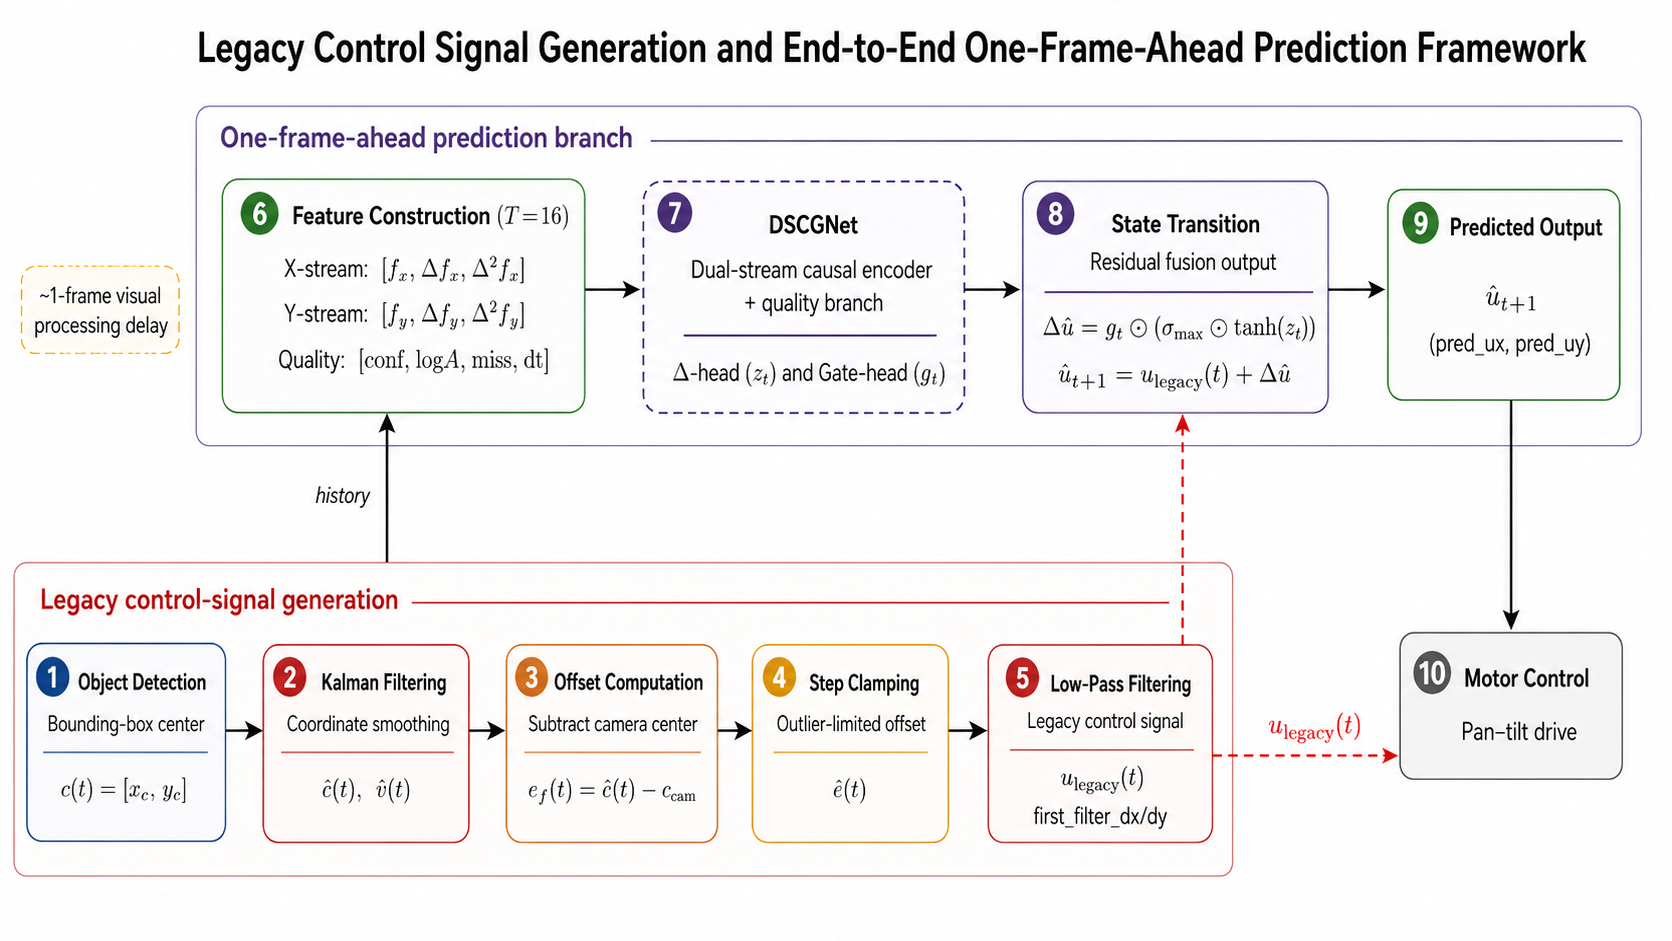
\includegraphics[width=0.95\textwidth]{picture/方法总体框架-1.png}
\caption{旧控制链生成与一帧超前基线控制参考预测框架。下半部分为已有工程基线控制链，上半部分为本文提出的因果时序预测分支。}
\label{fig:method_overview}
\end{figure*}

\subsection{特征构造}
对于每个时刻 $i$，模型输入特征由运动特征和质量特征组成。运动特征包括当前基线控制参考、一阶差分和二阶差分：
\begin{equation}
\mathbf{x}^{m}_i=[f_x(i),f_y(i),d_x(i),d_y(i),dd_x(i),dd_y(i)],
\end{equation}
其中
\begin{equation}
\begin{aligned}
f_x(i)&=u_x^L(i), & f_y(i)&=u_y^L(i),\\
d_x(i)&=f_x(i)-f_x(i-1), & d_y(i)&=f_y(i)-f_y(i-1),\\
dd_x(i)&=d_x(i)-d_x(i-1), & dd_y(i)&=d_y(i)-d_y(i-1).
\end{aligned}
\end{equation}
质量特征定义为
\begin{equation}
q(i)=[\mathrm{conf}(i),\log(\mathrm{area}(i)+1),\mathrm{miss\_flag}(i),dt(i)],
\end{equation}
其中 $\mathrm{conf}$ 表示检测置信度，$\mathrm{area}$ 表示目标框面积，$\mathrm{miss\_flag}$ 表示当前时刻是否存在缺失或异常观测，$dt$ 表示相邻记录时间间隔。完整输入为
\begin{equation}
\mathbf{x}_i=[\mathbf{x}^{m}_i,q(i)].
\end{equation}
当关闭质量分支时，模型仅使用 $\mathbf{x}^{m}_i$。

\subsection{双流因果时序编码网络}
DSCGNet 将运动特征按轴划分为两条分支：$x$ 流输入 $[f_x,d_x,dd_x]$，$y$ 流输入 $[f_y,d_y,dd_y]$。每条运动分支由两层因果一维卷积、GRU 和可选因果注意力组成：
\begin{equation}
\mathrm{Input}\rightarrow\mathrm{CausalConv}(d=1)\rightarrow\mathrm{CausalConv}(d=2)\rightarrow\mathrm{GRU}\rightarrow\mathrm{CausalAttn}.
\end{equation}
两层因果卷积用于提取局部运动趋势，膨胀卷积扩大感受野，GRU 建模更长时间依赖，因果注意力在不引入未来信息的条件下增强对关键历史时刻的利用。

若启用质量分支，则 $q(i)$ 先经过 \texttt{Linear(4$\rightarrow$16)} 映射，再由 \texttt{GRU(16$\rightarrow$16)} 编码为质量状态 $h_q$。两条运动分支输出 $h_x,h_y\in\mathbb{R}^{32}$，质量分支输出 $h_q\in\mathbb{R}^{16}$，拼接后得到融合表示
\begin{equation}
h=[h_x,h_y,h_q]\in\mathbb{R}^{80}.
\end{equation}
若关闭质量分支，则融合表示仅由 $h_x$ 与 $h_y$ 构成。网络结构如图\ref{fig:model_architecture}所示。

\begin{figure*}[!t]
\centering
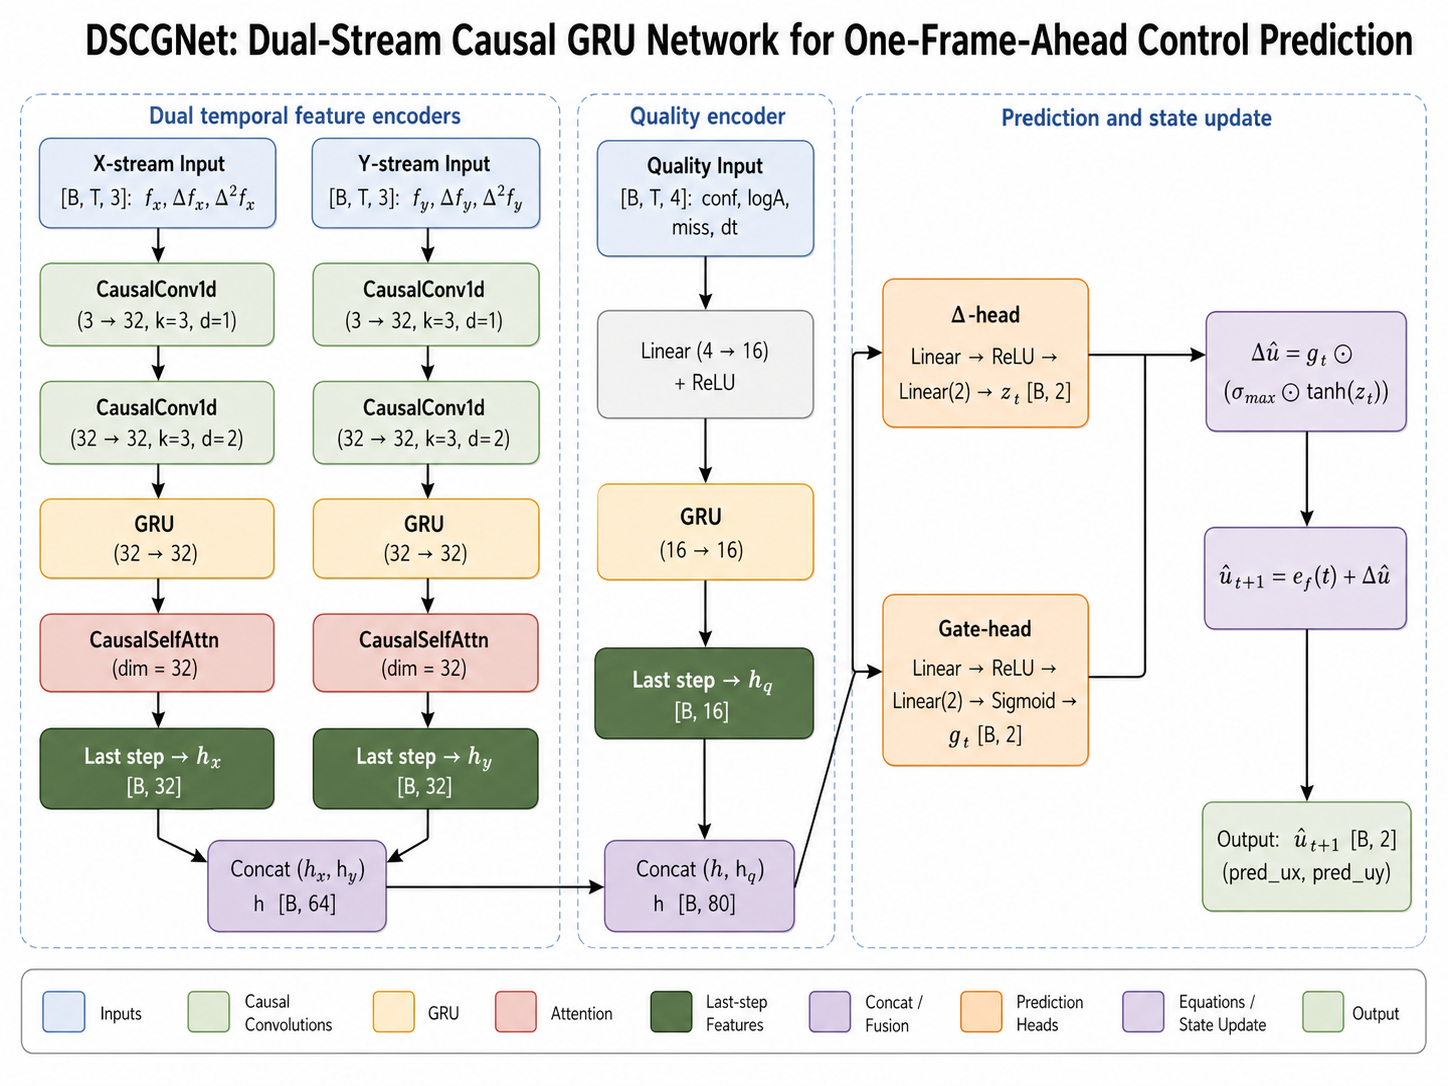
\includegraphics[width=0.95\textwidth]{picture/模型-1.png}
\caption{DSCGNet 模型架构。基础控制特征按 $x/y$ 轴分流编码，质量特征由独立分支建模，融合后通过有界状态转移输出头生成下一帧基线控制参考。}
\label{fig:model_architecture}
\end{figure*}

\subsection{有界状态转移输出}
直接回归下一帧绝对控制参考可能导致输出无约束跳变，不利于控制链路接入。为此，DSCGNet 采用状态转移参数化输出。融合表示 $h$ 经共享融合层后分别送入 delta head 和 gate head：
\begin{equation}
z_t=\phi_{\Delta}(h),\quad g_t=\sigma(\phi_g(h)),
\end{equation}
其中 $z_t\in\mathbb{R}^2$ 为候选增量，$g_t\in[0,1]^2$ 为门控系数。最终预测增量为
\begin{equation}
\Delta\hat{u}_t=g_t\odot\left(r_{\max}\odot\tanh(z_t)\right),
\end{equation}
预测控制参考为
\begin{equation}
\hat{u}^L(t+1)=u^L(t)+\Delta\hat{u}_t.
\end{equation}
其中 $r_{\max}=[12,12]$ 表示每个轴的最大单步补偿幅度，$\odot$ 表示逐元素乘法。该设计将网络输出限制在当前稳定基线参考附近，使预测失败时的风险低于无约束绝对值回归。

\subsection{训练目标与控制友好正则}
训练标签为下一帧基线控制参考：
\begin{equation}
u^{target}(t+1)=u^L(t+1).
\end{equation}
总损失定义为
\begin{equation}
\mathcal{L}=\lambda_1\mathcal{L}_{ahead}+\lambda_2\mathcal{L}_{inc}+\lambda_3\mathcal{L}_{stab}+\lambda_4\mathcal{L}_{dir}+\lambda_5\mathcal{L}_{gate}.
\end{equation}
其中一帧预测误差采用 Huber 损失：
\begin{equation}
\mathcal{L}_{ahead}=\mathrm{Huber}\!\left(\hat{u}^L(t+1),u^L(t+1)\right).
\end{equation}
增量空间辅助误差为
\begin{equation}
\mathcal{L}_{inc}=\left\|\Delta\hat{u}_t-\Delta u_t\right\|_1,
\end{equation}
其中真实单步变化为
\begin{equation}
\Delta u_t=u^L(t+1)-u^L(t).
\end{equation}
需要说明的是，$\mathcal{L}_{inc}$ 与预测误差在代数上密切相关，其作用不是引入独立的新监督目标，而是在增量空间中以 $L_1$ 形式强调单步状态转移误差，并与 Huber 型 $\mathcal{L}_{ahead}$ 互补。

状态相关平滑正则定义为
\begin{equation}
\begin{aligned}
m_t&=\left\|u^L(t)-u^L(t-1)\right\|_1,\\
w_t&=\exp(-m_t/\tau),\\
\mathcal{L}_{stab}&=w_t\left\|\Delta\hat{u}_t\right\|_1.
\end{aligned}
\end{equation}
该项在低运动状态下抑制不必要补偿。本文中的 ``stab'' 表示控制友好的平滑正则，并非严格意义上的闭环 Lyapunov 稳定性证明。

方向一致性损失为
\begin{equation}
\mathcal{L}_{dir}=\max\left(0,-\Delta\hat{u}_t\cdot\Delta u_t\right),
\end{equation}
用于减少预测增量与真实单步变化方向相反的情况。门控稀疏正则为
\begin{equation}
\mathcal{L}_{gate}=\|g_t\|_1,
\end{equation}
用于避免模型在无明显需要时过度开启补偿门控。实验中采用 $\lambda_1=1.0$、$\lambda_2=0.5$、$\lambda_3=0.1$、$\lambda_4=0.1$、$\lambda_5=0.01$，$\tau=12.0$。

\subsection{部署方式}
在线部署时，模型维护最近 $T$ 帧已经由旧控制链产生的 $u^L$ 和质量特征，并在每个控制更新时刻输出 $\hat{u}^L(t+1)$。若执行端还存在电机幅值、角速度或帧间变化率限制，可在模型输出之后继续施加与原控制链一致的饱和保护和 slew-rate limiter。该保护属于执行器安全接口，不改变本文的因果预测问题定义。

\section{实验设置}

\subsection{实验平台}
本文数据采集自二维转台视觉伺服反无人机实验系统。如图\ref{fig:platform}所示，系统由视觉采集端、二维云台执行机构和控制计算单元组成。视觉端实时采集目标图像，检测算法输出目标框中心坐标；旧控制链对检测结果进行卡尔曼滤波、中心偏差计算、阶跃限幅和低通滤波，生成 $u^L(t)$。本文实验主要评估基于真实硬件闭环系统运行日志的信号级一帧前瞻预测能力，而不是声称已经完成完整在线闭环控制性能对比。

\begin{figure}[!t]
\centering
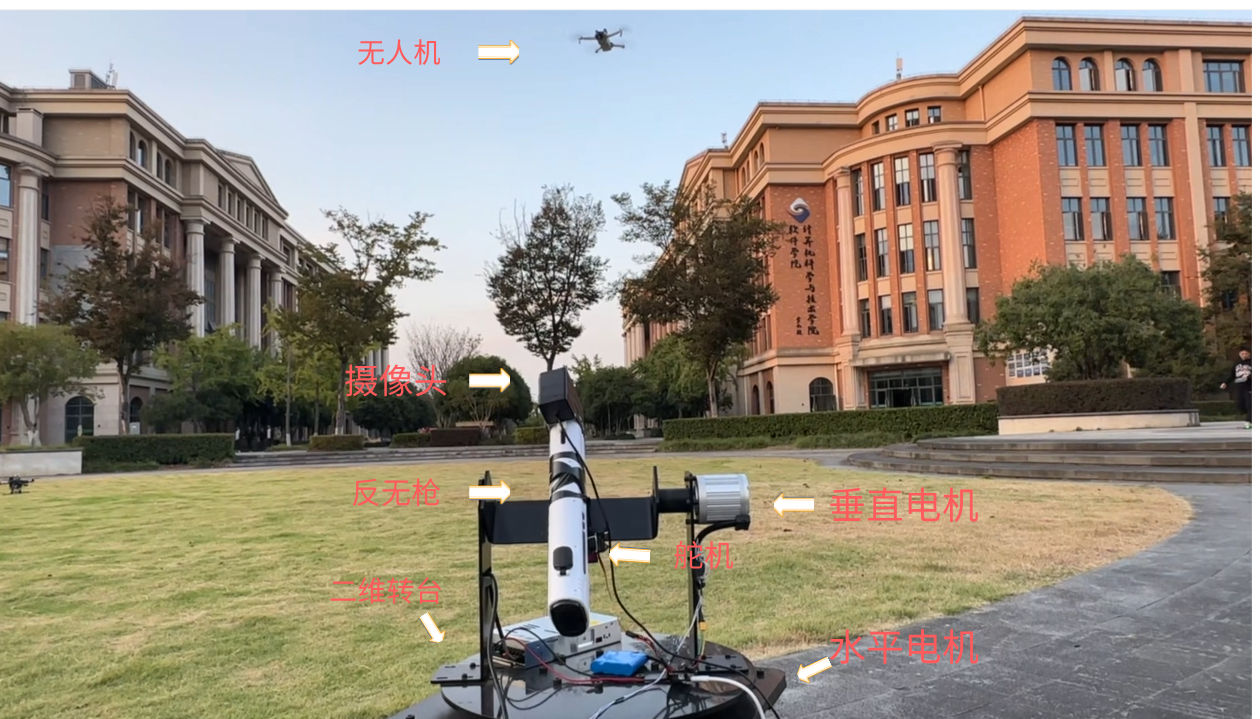
\includegraphics[width=0.48\textwidth]{picture/platform.png}
\caption{二维转台视觉伺服反无人机实验平台。本文数据来自该硬件系统的运行日志，实验评估重点为信号级下一帧控制参考预测。}
\label{fig:platform}
\end{figure}

\subsection{数据集}
实验数据来源于实际部署系统生成的数据日志文件 \path{track-fusion-move-baseline_new.csv}。其中 \path{first_filter_dx} 和 \path{first_filter_dy} 分别表示旧控制链输出的二维基线控制参考，即本文监督目标序列 $u^L(t)$ 的两个通道。

完整数据共包含 9451 条记录，覆盖 6 条轨迹。采用长度 $T=16$ 的滑动窗口构造样本后，共得到 9435 个有效样本，并按时间顺序划分为 6604 个训练样本、1415 个验证样本和 1416 个测试样本。数据集统计见表\ref{tab:dataset}。为避免对实验结果作过度外推，本文将当前验证范围限定为该批真实系统日志上的信号级预测；跨轨迹留一验证和更多场景泛化实验可作为后续补充。

\begin{table}[!t]
\centering
\caption{数据集统计}
\label{tab:dataset}
\begin{tabular}{lc}
\toprule
\textbf{Item} & \textbf{Value} \\
\midrule
Total records & 9451 \\
Trajectories & 6 \\
Effective samples & 9435 \\
Training set & 6604 (70\%) \\
Validation set & 1415 (15\%) \\
Test set & 1416 (15\%) \\
History length $T$ & 16 frames \\
Feature dimension & 10 (6 motion + 4 quality) \\
\bottomrule
\end{tabular}
\end{table}

\subsection{实现细节}
模型使用 PyTorch 实现，采用 AdamW 优化器，学习率 $10^{-3}$，权重衰减 $10^{-4}$，批大小 64。默认历史窗口长度为 $T=16$，启用质量分支和因果注意力，注意力头数为 4，dropout 为 0.1。状态转移输出中 $r_{\max}=[12,12]$。训练轮数设为 500，并根据验证集 Ahead MAE 保存最佳 checkpoint。完整模型参数量为 39\,284。

为评估部署效率，本文在 Intel Core i7-14700KF CPU、NVIDIA GeForce RTX 4070 Ti SUPER 16\,GB GPU 和 32\,GB 内存的实验电脑上测试单样本前向推理耗时。测试条件为 batch size 1、输入长度 $T=16$。统计仅包含模型前向推理，不包含图像采集和检测推理时间。

\subsection{评价指标}
令预测误差为
\begin{equation}
e_t=\hat{u}^L(t+1)-u^L(t+1),
\end{equation}
预测补偿增量和真实单步变化分别为
\begin{equation}
\Delta\hat{u}_t=\hat{u}^L(t+1)-u^L(t),\quad \Delta u_t=u^L(t+1)-u^L(t).
\end{equation}
本文采用如下指标：
\begin{equation}
\mathrm{MAE}=\frac{1}{N}\sum_{t=1}^{N}\|e_t\|_1,
\end{equation}
\begin{equation}
\mathrm{RMSE}=\sqrt{\frac{1}{2N}\sum_{t=1}^{N}\|e_t\|_2^2},
\end{equation}
\begin{equation}
\mathrm{Jitter}_{\Delta}=\frac{1}{N-1}\sum_{t=2}^{N}\|\Delta\hat{u}_t-\Delta\hat{u}_{t-1}\|_1,
\end{equation}
\begin{equation}
\mathrm{SpikeRate}=\frac{1}{N}\sum_{t=1}^{N}\mathbf{1}(\|e_t\|_2>\gamma_e),
\end{equation}
\begin{equation}
\mathrm{SignUnfollow}=\frac{1}{N}\sum_{t=1}^{N}\mathbf{1}\left(\mathrm{sgn}(\Delta\hat{u}_t)\neq \mathrm{sgn}(\Delta u_t)\right).
\end{equation}
其中 $\gamma_e$ 为误差突变阈值，$\mathrm{sgn}(\cdot)$ 按轴计算并按样本聚合。$\mathrm{Jitter}_{\Delta}$ 衡量的是补偿增量的抖动，而不是原始基线信号本身的抖动，因此 Last Value 方法的补偿增量恒为零时该指标为零。

\subsection{对比方法}
本文采用以下方法进行对比：
\begin{itemize}
    \item \textbf{Last Value}: $\hat{u}(t+1)=u^L(t)$，即不做前瞻补偿；
    \item \textbf{Linear Extrapolation}: $\hat{u}(t+1)=2u^L(t)-u^L(t-1)$，即基于一阶趋势的线性外推；
    \item \textbf{Kalman CV}: 采用常速度状态模型的卡尔曼滤波器，在当前时刻完成状态更新后执行一步预测；
    \item \textbf{GRU Direct}: 使用单流 GRU 直接回归下一帧绝对控制参考；
    \item \textbf{DSCGNet}: 本文提出的双流因果卷积、GRU、因果注意力、质量分支和状态转移参数化输出模型。
\end{itemize}

\section{结果与讨论}

\subsection{主要对比结果}
表\ref{tab:main_comparison}给出了测试集上的主要定量对比结果。

\begin{table}[!t]
\centering
\caption{主要方法对比（测试集）}
\label{tab:main_comparison}
\small
\setlength{\tabcolsep}{3pt}
\resizebox{\columnwidth}{!}{%
\begin{tabular}{lccccc}
\toprule
\textbf{方法} & \textbf{Ahead MAE} & \textbf{Ahead RMSE} & \textbf{Jitter$_\Delta$} & \textbf{Spike Rate} & \textbf{Sign Unfollow} \\
\midrule
Last Value & 1.7660 & 4.4408 & 0.0000 & 0.0212 & 1.0000 \\
Linear Extrapolation & 0.3135 & 4.7372 & 0.3137 & 0.0247 & 0.0275 \\
Kalman CV & 0.5643 & 6.0284 & 1.0566 & 0.0318 & 0.0307 \\
GRU Direct & 2.7794 & 9.1456 & 0.5465 & 0.0170 & 0.2066 \\
DSCGNet (本文方法) & \textbf{0.2157} & \textbf{3.3362} & 0.1903 & 0.0254 & \textbf{0.0258} \\
\bottomrule
\end{tabular}%
}
\end{table}

由表\ref{tab:main_comparison}可见，Last Value 不进行任何前瞻补偿，因此 Ahead MAE 较高。Linear Extrapolation 能够显著降低 MAE，说明基线控制参考序列中确实存在可利用的短时趋势；但其 RMSE 仍较高，表明简单线性外推在局部突变或非线性运动时容易产生较大误差。Kalman CV 相比 Last Value 有所改善，但其抖动和 RMSE 高于本文方法。GRU Direct 虽具备学习能力，但直接回归绝对控制参考在当前中小规模数据上表现不稳定。DSCGNet 在 Ahead MAE 和 Ahead RMSE 上取得最佳结果，同时保持较低的补偿增量抖动和方向未跟随率，说明有界状态转移输出和双流因果时序建模更适合该任务。

\subsection{测试集时序对比}
图\ref{fig:test_prediction}展示了测试集动态片段上各方法对下一帧基线控制参考的预测曲线，其中上下两个子图分别对应 $x$ 和 $y$ 通道。可以看出，DSCGNet 在整体趋势和局部变化上与真实下一帧控制参考保持较高一致性，并相较 Last Value 和 GRU Direct 减少了明显滞后或偏离。局部放大区域进一步显示，线性外推在部分变化段可能产生过冲，而本文方法因采用门控和有界增量输出，在保持前瞻性的同时具有更平滑的局部变化。

\begin{figure}[!t]
\centering
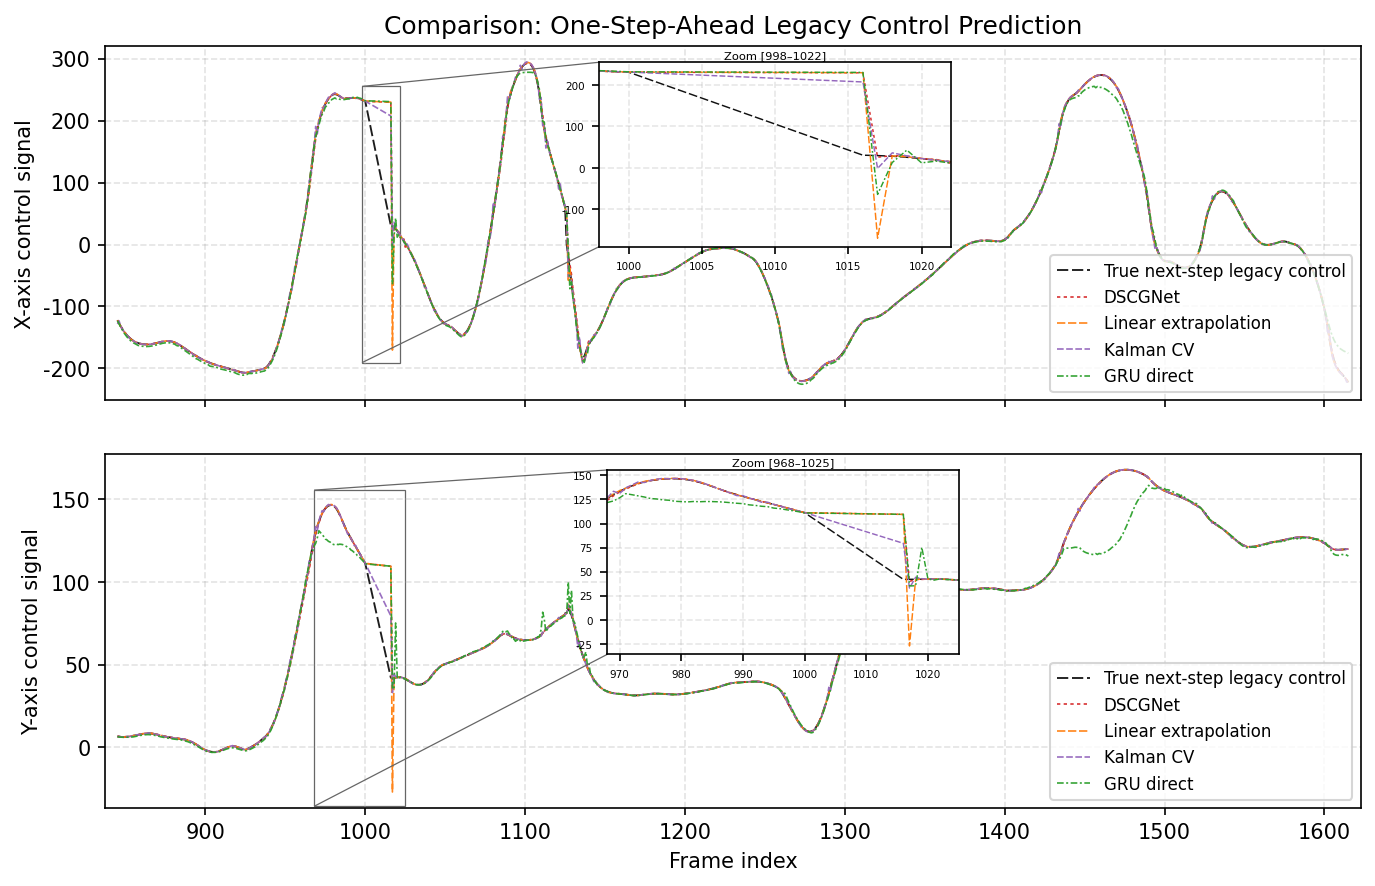
\includegraphics[width=0.48\textwidth]{picture/new_capture_2026_04_17_600pts/interactive_inset.png}
\caption{测试集动态片段上各方法下一帧控制参考预测结果对比及局部放大图。}
\label{fig:test_prediction}
\end{figure}

\subsection{结构消融分析}
为分析各结构因素的作用，本文围绕历史长度 $T$、质量分支、因果注意力和输出头形式进行消融实验。需要说明的是，表\ref{tab:ablation_results}来自独立消融实验协议，主要用于比较同一协议内不同结构选择的相对影响；由于当前消融实验与表\ref{tab:main_comparison}中的最终主实验 checkpoint 和评估脚本存在版本差异，表\ref{tab:ablation_results}中的绝对数值不与表\ref{tab:main_comparison}直接横向比较。后续定稿时建议使用统一脚本重跑主实验和消融实验。

\begin{table}[!t]
\centering
\caption{历史长度、质量分支、因果注意力与输出头消融结果（独立消融协议，测试集）}
\label{tab:ablation_results}
\small
\setlength{\tabcolsep}{3pt}
\resizebox{0.98\columnwidth}{!}{%
\begin{tabular}{llccc}
\toprule
\textbf{类别} & \textbf{设置} & \textbf{Ahead MAE} & \textbf{Ahead RMSE} & \textbf{Jitter$_\Delta$} \\
\midrule
历史长度 & $T=8$ & 0.8165 & 6.2868 & 2.8859 \\
历史长度 & $T=12$ & 0.8827 & 6.2967 & 2.8780 \\
历史长度 & $T=16$ & 0.7374 & 6.1753 & 2.9166 \\
历史长度 & $T=20$ & 1.0223 & 6.2838 & 2.9334 \\
质量分支 & 关闭 & 1.0664 & 6.3291 & 2.9568 \\
质量分支 & 开启 & 0.8374 & 6.2753 & 2.8361 \\
因果注意力 & 关闭 & 0.7808 & 6.2778 & 2.8614 \\
因果注意力 & 开启 & 0.6374 & 6.0753 & 2.8166 \\
输出头 & 直接回归输出 & 6.0408 & 11.9976 & 3.6696 \\
输出头 & 状态转移参数化输出 & 0.8022 & 6.2583 & 2.8491 \\
\bottomrule
\end{tabular}%
}
\end{table}

在表\ref{tab:ablation_results}的同一消融协议下，$T=16$ 在历史长度对比中取得较低 MAE 和 RMSE，说明过短历史窗口难以捕获足够运动趋势，而过长历史窗口可能引入冗余甚至过时信息。开启质量分支后，MAE、RMSE 和抖动均有所下降，说明置信度、目标尺度、丢帧标记和时间间隔等质量信息有助于判断历史控制参考的可靠性。因果注意力进一步降低误差，表明模型能够从历史窗口中选择与当前一步预测更相关的片段。输出头消融显示，直接回归绝对控制参考的误差显著高于状态转移参数化输出，说明以当前稳定控制参考为锚点预测有界增量是本文方法中的关键设计。

\subsection{模型复杂度与推理速度}
表\ref{tab:model_architecture_detail}给出了默认 DSCGNet 的结构细节和参数量。完整模型总参数量为 39\,284，其中主要参数来自两条运动时序编码分支和融合输出头，质量分支仅引入较小额外开销。

\begin{table}[!t]
\centering
\caption{所提 DSCGNet 的详细架构（质量分支开启）}
\label{tab:model_architecture_detail}
\small
\setlength{\tabcolsep}{2.5pt}
\resizebox{0.98\columnwidth}{!}{%
\begin{tabular}{lccc}
\toprule
\textbf{模块} & \textbf{配置} & \textbf{输出形状} & \textbf{参数量} \\
\midrule
X流输入 & $[f_x,d_x,dd_x]$ & [B,16,3] & 0 \\
Y流输入 & $[f_y,d_y,dd_y]$ & [B,16,3] & 0 \\
质量分支输入 & $[\mathrm{conf},\log(\mathrm{area}+1),\mathrm{miss\_flag},dt]$ & [B,16,4] & 0 \\
每流因果卷积1 & $3\rightarrow32$, $k=3$, $d=1$ & [B,16,32] & 320 / 流 \\
每流因果卷积2 & $32\rightarrow32$, $k=3$, $d=2$ & [B,16,32] & 3,104 / 流 \\
每流GRU & $32\rightarrow32$ & [B,16,32] & 6,336 / 流 \\
每流因果注意力 & dim=32, heads=4 & [B,16,32] & 4,288 / 流 \\
质量分支编码 & Linear$(4\rightarrow16)$ + GRU$(16\rightarrow16)$ & [B,16,16] & 1,712 \\
融合层 & Linear$(80\rightarrow64)$ + ReLU + Dropout & [B,64] & 5,184 \\
Delta head & Linear$(64\rightarrow32\rightarrow2)$ & [B,2] & 2,146 \\
Gate head & Linear$(64\rightarrow32\rightarrow2)$ & [B,2] & 2,146 \\
\midrule
\textbf{总计} & & & \textbf{39,284} \\
\bottomrule
\end{tabular}%
}
\end{table}

为避免推理速度口径不一致，本文统一采用表\ref{tab:latency}中的单样本前向推理统计。GPU 平均推理耗时约为 1.50\,ms，CPU 平均推理耗时约为 1.70\,ms。该耗时不包含图像采集和目标检测推理，但相对于 30\,FPS 系统中约 33\,ms 的帧周期较小，说明 DSCGNet 作为附加补偿模块具有较好的实时部署潜力。

\begin{table}[!t]
\centering
\caption{单样本前向推理速度（batch size 1，$T=16$）}
\label{tab:latency}
\begin{tabular}{lcc}
\toprule
\textbf{设备} & \textbf{平均耗时} & \textbf{等效频率} \\
\midrule
NVIDIA RTX 4070 Ti SUPER 16\,GB & 1.50\,ms & 664.68\,Hz \\
Intel Core i7-14700KF & 1.70\,ms & 588.56\,Hz \\
\bottomrule
\end{tabular}
\end{table}

\subsection{方法优势与局限性}
本文方法的主要优势包括：首先，预测目标来自已有工程基线控制链，避免直接从原始图像到执行器命令的高风险端到端替代；其次，双流因果时序编码和质量分支能够同时利用运动趋势与观测可靠性；再次，有界状态转移输出使网络以当前稳定控制参考为锚点生成受限补偿增量，更适合与原控制链融合；最后，模型规模较小，推理耗时低，满足实时补偿模块的基本要求。

本文也存在局限。第一，当前数据规模仍为中小规模，覆盖 6 条轨迹，模型泛化能力还需要通过更多轨迹、不同环境和不同目标运动模式验证。第二，本文主要评估信号级 one-step-ahead prediction，尚未系统报告接入完整在线闭环后的跟踪误差、超调、稳定时间和丢靶率等指标。第三，当前方法针对一帧级滞后设计，若视觉链路时延显著增加或帧率变化较大，需要重新校准窗口长度、$r_{\max}$ 和输出接口。第四，消融实验当前仍应使用统一训练与评估脚本进一步复核，以提高最终论文的实验一致性。

\section{结论}
本文针对视觉伺服反无人机系统中由图像采集、目标检测推理和控制信号整形共同引起的一帧级滞后问题，提出了一种轻量因果时序网络 DSCGNet。与直接预测图像目标位置或端到端替代底层控制器不同，本文将时延补偿表述为已有基线控制参考信号的严格因果一帧超前预测。该问题定义使学习目标直接对应真实工程控制链中的稳定参考量，有利于降低部署风险。

方法上，DSCGNet 利用历史基线控制参考、一阶差分、二阶差分和检测质量特征构造输入，通过 $x/y$ 双流因果卷积、GRU、因果注意力和质量分支提取时序表示，并采用有界状态转移参数化输出头生成下一帧控制参考。训练目标同时考虑一帧预测误差、增量空间辅助误差、状态相关平滑正则、方向一致性和门控稀疏性，使输出更符合控制链路对平滑性和受限变化的要求。

基于真实二维转台视觉伺服反无人机系统日志的信号级实验表明，DSCGNet 在 Ahead MAE 和 Ahead RMSE 上优于 Last Value、Linear Extrapolation、Kalman CV 和 GRU Direct 等基线，同时保持较低的补偿增量抖动和方向未跟随率。结构消融进一步表明，质量分支、因果注意力和状态转移参数化输出对模型性能具有积极作用。未来工作将重点补充统一口径的消融实验、跨轨迹泛化验证和完整在线闭环控制评估，以进一步量化该补偿模块对实际跟踪性能的提升。

\begin{thebibliography}{30}

\bibitem{chaumette2006visual}
F.~Chaumette and S.~Hutchinson, ``Visual servo control. I. Basic approaches,'' \emph{IEEE Robotics \& Automation Magazine}, vol.~13, no.~4, pp. 82--90, 2006.

\bibitem{hutchinson1996tutorial}
S.~Hutchinson, G.~D. Hager, and P.~I. Corke, ``A tutorial on visual servo control,'' \emph{IEEE Transactions on Robotics and Automation}, vol.~12, no.~5, pp. 651--670, 1996.

\bibitem{corke2011robotics}
P.~Corke, \emph{Robotics, Vision and Control: Fundamental Algorithms in MATLAB}. Springer, 2011.

\bibitem{yilmaz2006object}
A.~Yilmaz, O.~Javed, and M.~Shah, ``Object tracking: A survey,'' \emph{ACM Computing Surveys}, vol.~38, no.~4, p. 13, 2006.

\bibitem{redmon2016you}
J.~Redmon, S.~Divvala, R.~Girshick, and A.~Farhadi, ``You only look once: Unified, real-time object detection,'' in \emph{Proc. IEEE Conference on Computer Vision and Pattern Recognition}, 2016, pp. 779--788.

\bibitem{he2016deep}
K.~He, X.~Zhang, S.~Ren, and J.~Sun, ``Deep residual learning for image recognition,'' in \emph{Proc. IEEE Conference on Computer Vision and Pattern Recognition}, 2016, pp. 770--778.

\bibitem{ren2015faster}
S.~Ren, K.~He, R.~Girshick, and J.~Sun, ``Faster R-CNN: Towards real-time object detection with region proposal networks,'' arXiv preprint arXiv:1506.01497, 2015.

\bibitem{bochkovskiy2020yolov4}
A.~Bochkovskiy, C.-Y. Wang, and H.-Y.~M. Liao, ``YOLOv4: Optimal speed and accuracy of object detection,'' arXiv preprint arXiv:2004.10934, 2020.

\bibitem{carion2020detr}
N.~Carion, F.~Massa, G.~Synnaeve, N.~Usunier, A.~Kirillov, and S.~Zagoruyko, ``End-to-end object detection with transformers,'' in \emph{European Conference on Computer Vision}. Springer, 2020, pp. 213--229.

\bibitem{cao2022survey_cn}
曹家乐, 李亚利, 孙汉卿, 谢今, 黄凯奇, and 庞彦伟, ``基于深度学习的视觉目标检测技术综述,'' \emph{中国图象图形学报}, vol.~27, no.~6, pp. 1697--1722, 2022.

\bibitem{leng2023droneview_cn}
冷佳旭, 莫梦竟成, 周应华, 叶永明, 高陈强, and 高新波, ``无人机视角下的目标检测研究进展,'' \emph{中国图象图形学报}, vol.~28, no.~9, pp. 2563--2586, 2023.

\bibitem{shi2021anti}
X.~Shi, C.~Yang, W.~Xie, C.~Liang, Z.~Shi, and J.~Chen, ``Anti-drone system with multiple surveillance technologies: Architecture, implementation, and challenges,'' \emph{IEEE Communications Magazine}, vol.~56, no.~4, pp. 68--74, 2018.

\bibitem{kalman1960new}
R.~E. Kalman, ``A new approach to linear filtering and prediction problems,'' \emph{Journal of Basic Engineering}, vol.~82, no.~1, pp. 35--45, 1960.

\bibitem{welch1995introduction}
G.~Welch and G.~Bishop, ``An introduction to the Kalman filter,'' University of North Carolina at Chapel Hill, Department of Computer Science, Tech. Rep., 1995.

\bibitem{smith1957closer}
O.~J. Smith, ``Closer control of loops with dead time,'' \emph{Chemical Engineering Progress}, vol.~53, no.~5, pp. 217--219, 1957.

\bibitem{camacho2013model}
E.~F. Camacho and C.~B. Alba, \emph{Model Predictive Control}. Springer, 2013.

\bibitem{lecun2015deep}
Y.~LeCun, Y.~Bengio, and G.~Hinton, ``Deep learning,'' \emph{Nature}, vol. 521, no. 7553, pp. 436--444, 2015.

\bibitem{hochreiter1997long}
S.~Hochreiter and J.~Schmidhuber, ``Long short-term memory,'' \emph{Neural Computation}, vol.~9, no.~8, pp. 1735--1780, 1997.

\bibitem{cho2014learning}
K.~Cho, B.~van Merriënboer, C.~Gulcehre, D.~Bahdanau, F.~Bougares, H.~Schwenk, and Y.~Bengio, ``Learning phrase representations using RNN encoder-decoder for statistical machine translation,'' arXiv preprint arXiv:1406.1078, 2014.

\bibitem{bai2018empirical}
S.~Bai, J.~Z. Kolter, and V.~Koltun, ``An empirical evaluation of generic convolutional and recurrent networks for sequence modeling,'' arXiv preprint arXiv:1803.01271, 2018.

\bibitem{normey2009taking}
J.~E. Normey-Rico and E.~F. Camacho, ``Taking the controller apart: On the need of model-free control theory,'' \emph{IFAC Proceedings Volumes}, vol.~42, no.~11, pp. 139--144, 2009.

\bibitem{xi2013mpc_cn}
席裕庚, 李德伟, and 林姝, ``模型预测控制---现状与挑战,'' \emph{自动化学报}, vol.~39, no.~3, pp. 222--236, 2013.

\bibitem{li2006saturatedmpc_cn}
李志军, 刘吉臻, and 谭文, ``饱和约束系统的鲁棒模型预测控制,'' \emph{控制与决策}, vol.~21, no.~6, pp. 641--645, 2006.

\bibitem{chen2007timedelaympc_cn}
陈秋霞 and 俞立, ``不确定离散时滞系统的输出反馈鲁棒预测控制,'' \emph{控制理论与应用}, vol.~24, no.~3, pp. 401--406, 2007.

\bibitem{liu2003advancedpid}
刘金琨, \emph{先进 PID 控制及其 MATLAB 仿真}. 北京: 电子工业出版社, 2003.

\bibitem{oord2016wavenet}
A.~van den Oord, S.~Dieleman, H.~Zen, K.~Simonyan, O.~Vinyals, A.~Graves, N.~Kalchbrenner, A.~Senior, and K.~Kavukcuoglu, ``WaveNet: A generative model for raw audio,'' arXiv preprint arXiv:1609.03499, 2016.

\bibitem{qin2017darnn}
Y.~Qin, D.~Song, H.~Chen, W.~Cheng, G.~Jiang, and G.~W. Cottrell, ``A dual-stage attention-based recurrent neural network for time series prediction,'' in \emph{Proc. International Joint Conference on Artificial Intelligence}, 2017, pp. 2627--2633.

\bibitem{lim2021tft}
B.~Lim, S.~Ö. Arik, N.~Loeff, and T.~Pfister, ``Temporal fusion transformers for interpretable multi-horizon time series forecasting,'' \emph{International Journal of Forecasting}, vol.~37, no.~4, pp. 1748--1764, 2021.

\bibitem{vaswani2017attention}
A.~Vaswani, N.~Shazeer, N.~Parmar, J.~Uszkoreit, L.~Jones, A.~N. Gomez, Ł.~Kaiser, and I.~Polosukhin, ``Attention is all you need,'' in \emph{Advances in Neural Information Processing Systems}, 2017, pp. 5998--6008.

\bibitem{wen2023transformers}
Q.~Wen, T.~Zhou, C.~Zhang, W.~Chen, Z.~Ma, J.~Yan, and L.~Sun, ``Transformers in time series: A survey,'' arXiv preprint arXiv:2202.07125, 2023.

\end{thebibliography}

\end{document}
